\section{Results}
\label{sec:results}

We wrote a simple CLI program to evaluate the algorithm under different conditions.
The program allows to set the input dimensions, the number of errors to introduce
and whether they should be collinear or not,
the simulated maximum amount of global memory, and the buffering strategy to use.
Several minor debugging parameters can be set, but they are out of the scope of this paper.

We tested the four strategies on a Quadro K620 desktop GPU. An important thing to consider is that display GPUs have a timeout on kernel executions, so we couldn't run tests with very large matrices. In any case, we believe that for bigger matrices the calculated performance should increase asymptotically.

When it came to profiling, the Nsight Compute suite was only available for the newer Ampere architecture, and for this GPU (Maxwell architecture), nvprof didn't have support for performance counters. For this reason we embedded some sort of profiling in the program itself.

As performance metrics, we used the overall execution time of the program (both total CPU and CUDA only), the total floating point arithmetic intensity and the average program performance (calculated as the total floating point operations over the total CUDA time).

To calculate the total floating point operations and the associated transfers to and from global memory (to then calculate the arithmetic intensity), we manually calculated the floating point operations number and associated global memory transfers count for each kernel we wrote. The program registers each kernel call and adds its float operations and transfers count to their respective counter.

To calculate the effective compute time we use CUDA events to register the start and end of the program (getting the total CUDA time with respect to the default stream).
To calculate the average performance we divide the total float operations by the total CUDA time, as a higher value indicate a higher use of the compute queue.
To calculate the total intensity we divide the total float operations by the total transfer count.

With that said, we hereby present our considerations on the obtained results.
We launched the same multiplication for the four different strategies, with inputs $20000 \times 2000$ and $2000 \times 2000$ (around 320MB of required memory), with the available global memory constrained to 10MB.

\begin{figure}[h]
  \centering
  \minipage{.481\textwidth}
  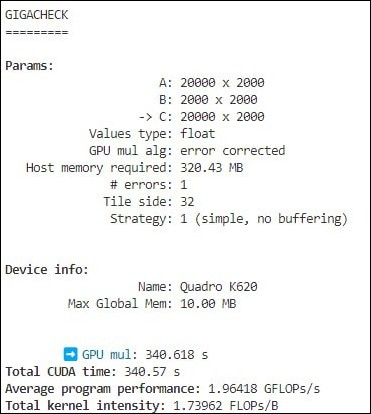
\includegraphics[width=\textwidth]{images/result_s1}
  \caption*{Strategy 1}
  \endminipage\hfill
  \minipage{.49\textwidth}
  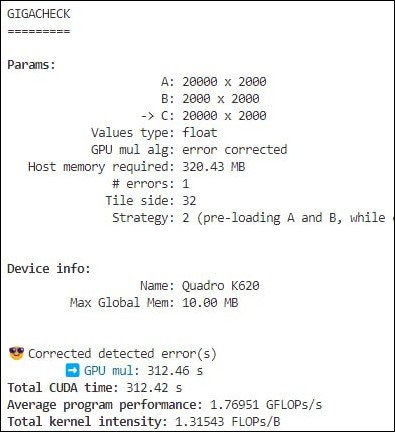
\includegraphics[width=\textwidth]{images/result_s2}
  \caption*{Strategy 2}
  \endminipage\hfill
  \linebreak
  \vspace{.02\textwidth}
  \linebreak
  \minipage{.481\textwidth}
  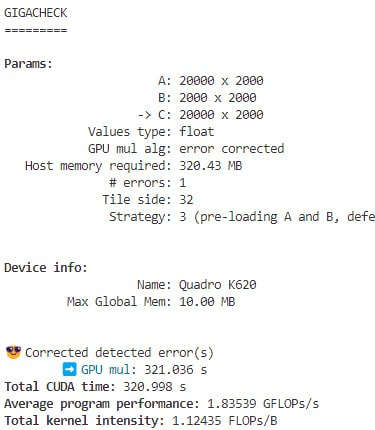
\includegraphics[width=\textwidth]{images/result_s3}
  \caption*{Strategy 3}
  \endminipage\hfill
  \minipage{.49\textwidth}
  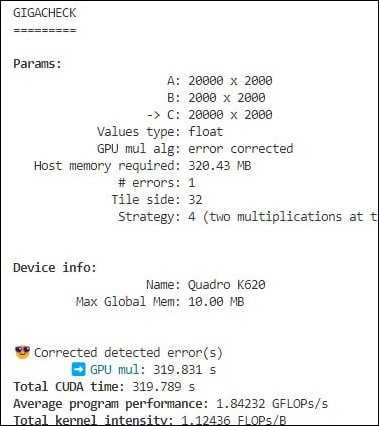
\includegraphics[width=\textwidth]{images/result_s4}
  \caption*{Strategy 4}
  \endminipage\hfill
  \caption{\centering results for the different strategies}\label{img:results-strategies}
\end{figure}

\img{ranking}{0.5\linewidth}{strategies ranking based on extracted metrics}

We see that, in comparison to strategy 1, strategy 2 has a slightly worse performance and intensity, but takes less overall time, as conjectured in \ref{img:strategies-timing-diagram}.

Strategy 3 has a slightly worse performance but less time than strategy 1, but higher performance than strategy 2 at a slightly higher time. The intensity is the lowest among all strategies.
Strategy 4 has a very similar intensity to strategy 2, but showing the best performance of all strategies as expected from the compute queue utilization maximization hypothesis. However, from the execution time we can tell we are between the best and worst case scenarios for this strategy. We can motivate this due to our imperfect implementation of the depth-first cuda calls scheduling, which doesn't allow an exactly concurrent H2D copy with one of the multiplication kernels.

One could ask why some strategies have higher average performance while taking more time than other strategies with lower performance. We can answer this by observing that the average performance is an indicator of the overall compute queue utilization, being the ratio of the total floating point operations (hardcoded) over the total execution time (including PCIe transfers). A strategy that has higher average performance means either that it is keeping the compute queue occupied more than the copy queues, or that there is an efficient concurrency between copies and computation. However, as we've seen in the \hyperref[sec:strategies]{Strategies section}, a strategy with less gaps between kernel execution must process lower sized blocks, and perform more transfers before processing the whole matrix, thus we can conclude that the overall execution time is a tradeoff between occupancy and block size.

Another thing that could seem counterintuitive is why strategy 1 has the highest intensity but is the slowest overall. We can motivate this by recalling that the intensity is hardcoded as the ratio of the total registered floating point operations count over the total registered bytes amount, so it is not dependent on time. Strategy 1 has to work on bigger blocks since it does not have auxiliary buffers. This enables it to make better use of the memory transfer, by being able to load less times the same blocks. Consequently, it is able to perform the same number of operations with less memory transfers, and that is what raises its intensity. However, the transfers it has to make are bigger and thus slower with respect to less intense strategies, and there are more and larger gaps between kernel executions.

\begin{figure}[h]
  \centering
  \minipage{.49\textwidth}
  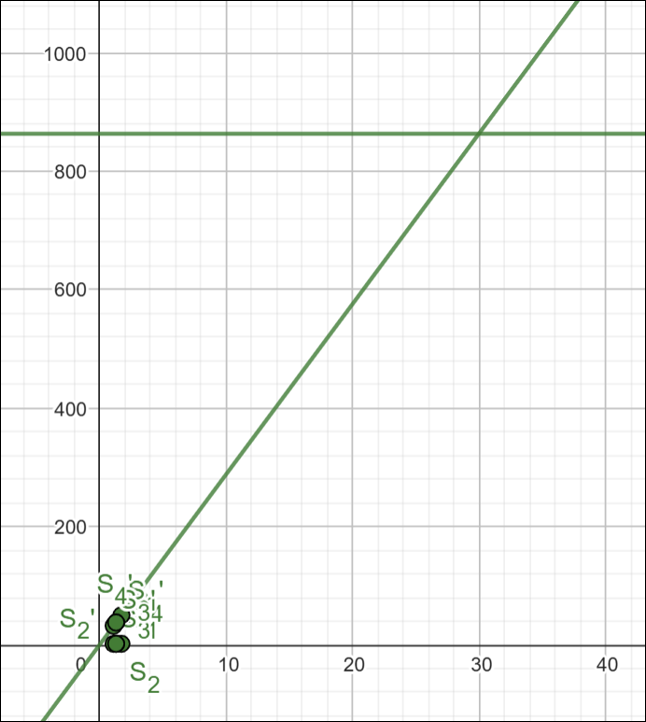
\includegraphics[width=\textwidth]{images/roofline-overview}
  \caption*{(a)}
  \endminipage\hfill
  \minipage{.49\textwidth}
  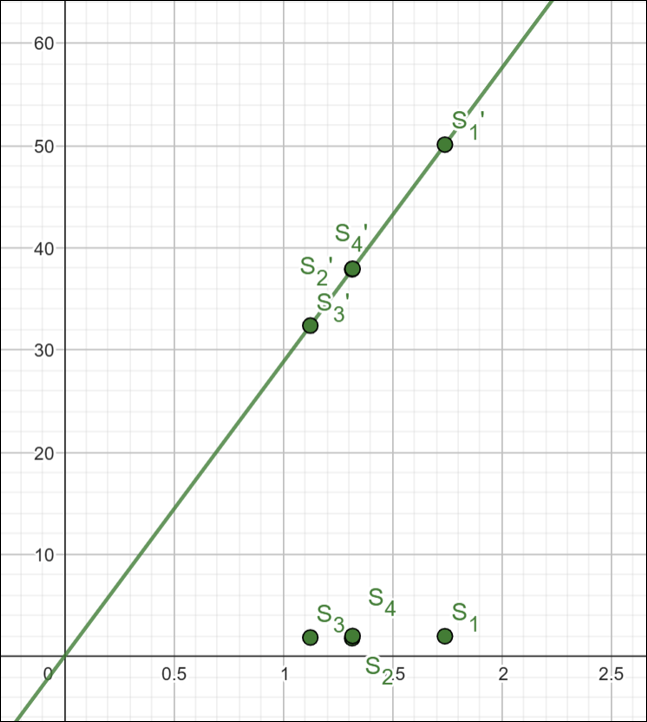
\includegraphics[width=\textwidth]{images/roofline-zoom.png}
  \caption*{(b)}
  \endminipage\hfill
  \caption{\centering naive roofline model, (a) complete and (b) zoomed on the area where our program stands}\label{img:roofline-model}
\end{figure}

Finally,
we plotted our results in the naive roofline model for this GPU in \ref{img:roofline-model}. We plotted the average performance points ($S_x$, which reflect the real observed performance), as well as the naive performance ($S_x'$) we would have according to the naive roofline model, that we obtained multiplying the total registered intensity by the maximum declared bandwidth of the GPU. The naive performance points lie higher on the graph than the observed ones. We observe that the naive performance differs not only in value, but also in the final ranking of the strategies with respect to the real observed performance.
